\section{Community structure and bridge nodes}
\label{sec:facebook-community}

Following the team protocol, we used the canonical edge list and original-graph
centrality rankings released by Member A. The graph derives from the
\href{https://snap.stanford.edu/data/ego-Facebook.html}{SNAP Facebook ego-network
collection} of \citet{mcauley2012social}. It contains
4,039 anonymized accounts and 88,234 undirected, unweighted friendship edges,
with the original integer node IDs preserved.

\subsection{Louvain communities}

Louvain greedily optimizes modularity by reassigning nodes and aggregating
groups \citep{blondel2008fast}. We used NetworkX~3.3 with unit edge weights,
resolution \(1\), convergence threshold \(10^{-7}\), and seed 602610. The
partition contained 16 communities ranging from 19 to 548 nodes
(Figure~\ref{fig:facebook-sizes}). Modularity was \(Q=0.835\), and 84,787
edges (96.09\%) were within a community. The partition thus provides a coarse
view of where friendship ties concentrate.

\begin{figure}[tbp]
  \centering
  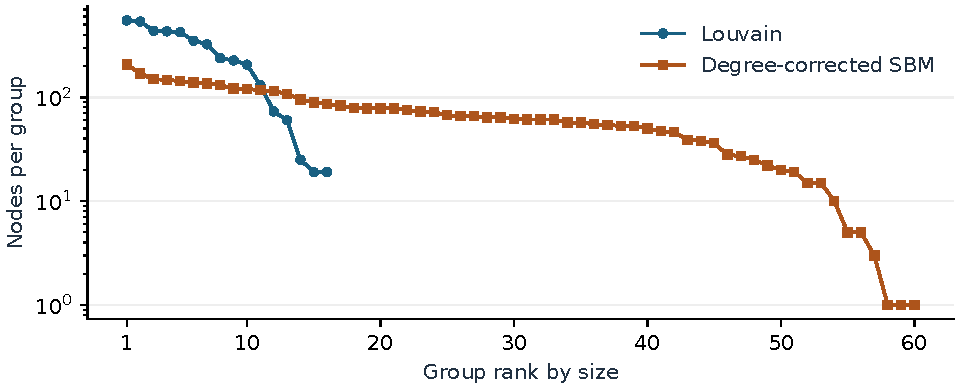
\includegraphics[width=0.9\linewidth]{partition_sizes.pdf}
  \caption{Group sizes in descending order. The vertical axis is logarithmic.
  The SBM resolves more groups and includes three singleton blocks.}
  \label{fig:facebook-sizes}
\end{figure}

\subsection{Degree-corrected stochastic block model}

The degree-corrected SBM accounts for degree variation within a group while
estimating how groups connect \citep{karrer2011stochastic}. We fit an undirected
single-level \texttt{BlockState} with \texttt{deg\_corr=True} using
\texttt{graph-tool}~3.9. We ran \texttt{minimize\_blockmodel\_dl} on one CPU
thread for each of five seeds \citep{peixoto2014efficient}. We selected the
lowest description length returned by \texttt{state.entropy()}, with ties
resolved by the smaller seed. Table~\ref{tab:facebook-sbm-trials} gives all
five fits. The selected fit contained 60 occupied blocks with sizes from 1
to 206. The subgraphs induced by 17 of the 60 blocks were disconnected,
illustrating that a block can group nodes with similar connection patterns.

\begin{table}[tbp]
  \caption{Single-level degree-corrected SBM fits. Seed 602620 produced the
  shortest description length among the five runs.}
  \label{tab:facebook-sbm-trials}
  \centering
  \begin{tabular}{rrr}
    \toprule
    Seed & Description length (nats) & Occupied blocks\\
    \midrule
    \textbf{602620} & \textbf{206,159.845} & \textbf{60}\\
    602621 & 206,343.629 & 60\\
    602622 & 206,927.475 & 62\\
    602623 & 206,554.943 & 64\\
    602624 & 207,065.559 & 61\\
    \bottomrule
  \end{tabular}
\end{table}

For blocks \(r\) and \(s\) with sizes \(n_r\) and \(n_s\), let \(m_{rs}\)
count observed edges between them, counting each undirected edge once. We
computed \(m_{rs}/(n_r n_s)\) across distinct blocks and
\(m_{rr}/\binom{n_r}{2}\) within a block. Within-block density is undefined
for a singleton. Of the 1,770 distinct off-diagonal block pairs, 1,433
(81.0\%) shared zero edges. Within-block edges accounted for 64.55\% of all
edges (Figure~\ref{fig:facebook-density}).

\begin{figure}[tbp]
  \centering
  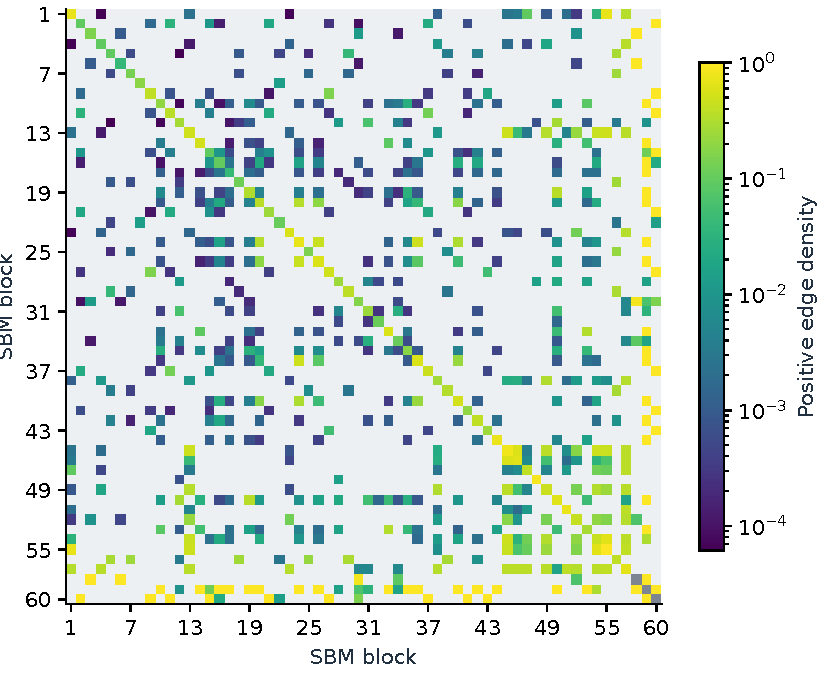
\includegraphics[width=0.74\linewidth]{block_connectivity_heatmap.pdf}
  \caption{Empirical SBM block-pair densities. The color scale is logarithmic
  for positive densities. Pale gray marks zero edges, and dark gray marks
  undefined singleton diagonals. A dense pair can represent few edges when
  one or both blocks are small.}
  \label{fig:facebook-density}
\end{figure}

\subsection{Agreement between the partitions}

We compared memberships on the same 4,039 nodes using the adjusted Rand
index, which corrects pairwise agreement for chance \citep{hubert1985comparing}.
The adjusted Rand index was 0.374. The largest Louvain community was spread
across eight SBM blocks, with its two largest contributions containing 143 and
136 members. Louvain communities 12 through 16 each lay within a single
SBM block (Figure~\ref{fig:facebook-overlap}). The two partitions agree on
some local groups and provide different resolutions of the larger groups.

\begin{figure}[tbp]
  \centering
  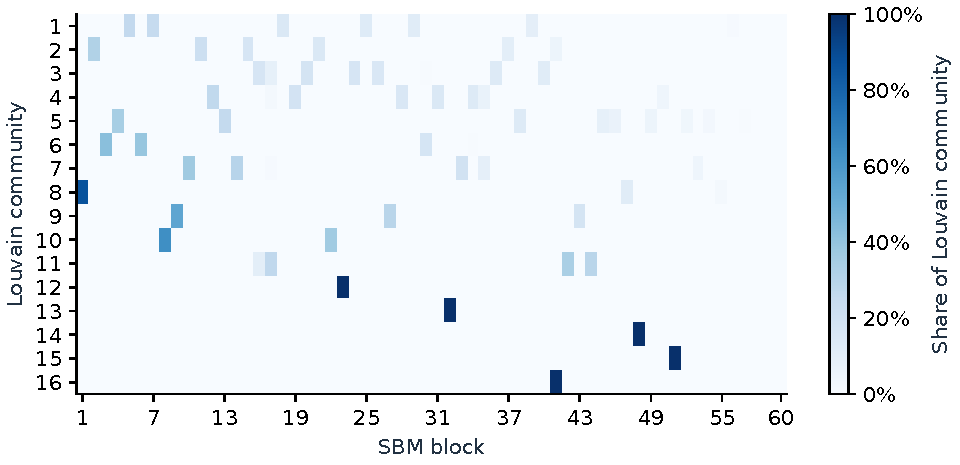
\includegraphics[width=0.92\linewidth]{partition_overlap.pdf}
  \caption{Membership overlap between Louvain and SBM. Each row sums to
  100\%. A dark cell indicates that one block contains a large fraction of
  that Louvain community.}
  \label{fig:facebook-overlap}
\end{figure}

\subsection{Bridge profiles of the highest-ranked nodes}

For each of the two Top-20 sets from the shared rankings, we measured the
number and fraction of a node's incident edges that connect to another
community or block. Fractions were computed per node and averaged with
equal weight for each node. The two lists shared 10 nodes. We retained
those nodes in each Top-20 mean and examined the disjoint subsets separately.
Each ranking occupied eight Louvain communities. The PageRank and
betweenness sets occupied 14 and 16 SBM blocks, respectively.

\begin{table}[tbp]
  \caption{Mean fractions and counts of a node's incident edges crossing
  Louvain communities or SBM blocks. Each node receives equal weight.}
  \label{tab:facebook-bridges}
  \centering
  \begin{tabular}{lrrrrr}
    \toprule
    & & \multicolumn{2}{c}{Cross-community} & \multicolumn{2}{c}{Cross-block}\\
    \cmidrule(lr){3-4}\cmidrule(l){5-6}
    Node set & \(n\) & Share (\%) & Count & Share (\%) & Count\\
    \midrule
    PageRank Top-20    & 20 & 10.36 & 66.75 & 57.56 & 225.95\\
    Betweenness Top-20 & 20 & 22.46 & 71.05 & 68.95 & 225.00\\
    PageRank only      & 10 &  4.43 &  9.00 & 45.56 &  70.70\\
    Betweenness only   & 10 & 28.62 & 17.60 & 68.35 &  68.80\\
    Both lists         & 10 & 16.29 & 124.50 & 69.55 & 381.20\\
    All nodes          & 4,039 & 4.16 & 1.71 & 30.19 & 15.49\\
    \bottomrule
  \end{tabular}
\end{table}

The betweenness Top-20 had higher mean crossing fractions at both
resolutions, and it reached more distinct external blocks per node on average
(8.60 versus 7.10). Absolute cross-block counts were nearly equal
(Table~\ref{tab:facebook-bridges}). Figure~\ref{fig:facebook-bridging} shows
the spread of these fractions across nodes. In the disjoint subsets,
PageRank-only nodes had higher mean degree (117.3 versus 81.5), while
betweenness-only nodes devoted a larger share of those ties to external groups.

The shared high-degree nodes also played prominent bridging roles. Node 107 ranked
first by betweenness and second by PageRank, with 611 of 1,045 ties crossing
communities and 1,045 crossing blocks. Its SBM block was a singleton, so a
100\% cross-block share follows from its assignment. Its 611 cross-community
ties provide separate evidence of its reach across the coarser partition.

\begin{figure}[tbp]
  \centering
  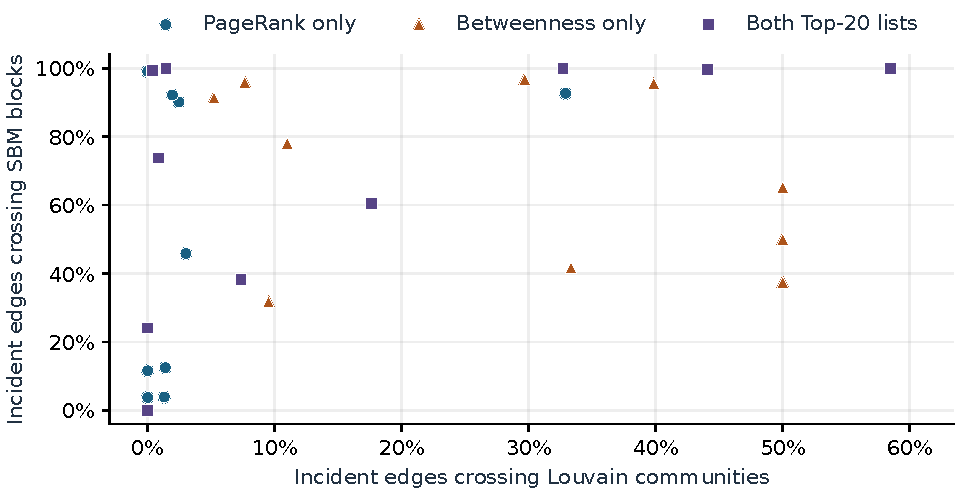
\includegraphics[width=0.94\linewidth]{top20_bridging.pdf}
  \caption{Per-node bridge profiles. Each distinct node in either ranking
  contributes one point. The marker distinguishes PageRank-only,
  betweenness-only, and shared nodes.}
  \label{fig:facebook-bridging}
\end{figure}

These profiles indicate that the betweenness ranking places a greater share
of ties across groups, which offers a structural explanation to examine
alongside the seeding and removal experiments. A topological crossing is a
potential route. Activation also depends on the seed set, the propagation
probability, and alternate paths. Our conclusions describe the sampled,
static graph, and the inferred groups are based solely on friendship edges.
